\documentclass[12pt,a4paper]{article} 
\usepackage[portuguese]{babel} \usepackage[utf8]{inputenc}
\usepackage{amsmath} 
\usepackage{graphicx}
\usepackage{booktabs}
\usepackage{float}
\begin{document}
\setcounter{figure}{2}
\setcounter{section}{3}
\setcounter{page}{4}
\section{Relatório}
\subsection{Introdução}

Nesta prática, deseja-se entender o funcionamento de um circuito integrado temporizador \emph{LM555}, e suas aplicações como um multivibrador monoestável e como um multivibrador astável (cirucito oscilador). 

Um vibrador monoestável é um circuito eletrônico que gera um pulso de saída. Quando desencadeado, um pulso de duração pré-defnida é produzido.
O circuito então retorna para seu estado de repouso e não produz outro sinal de saída até ser desencadeado novamente.

Um multivibrador é um circuito eletrônico usado para implementar uma variedade de dispositivos simples de dois estados como osciladores de relaxação, timers e flip-flops.
Ele consiste de dois dispositivos amplificadores (transistores, tubos de vácuo ou outros dispositivos) acoplado com resistores e capacitores.
O primeiro circuito multivibrador, o circuito multivibrador astável, foi inventado por Henri Abraham e Eugene Bloch durante a primeira guerra mundial. 
Eles chamaram de circuito multivibrador pois a forma de onda da saída era rica em harmônicos. 
Já um multivibrador astável é um circuito que não está estável em nenhum estado; continuamente troca de um estado para outro. Este funciona como oscilador de relaxação.

No experimento, o circuito integrado LM555 foi escolhido pois ele pode operar tanto como em uma configuração monoestável e astável. O diagrama descrito pela Figura~\ref{fig:0} acompanhado da Tabela~\ref{tab:1} evidenciam as funções que cada pino exerce.

\begin{figure}[htpb]
  \centering
  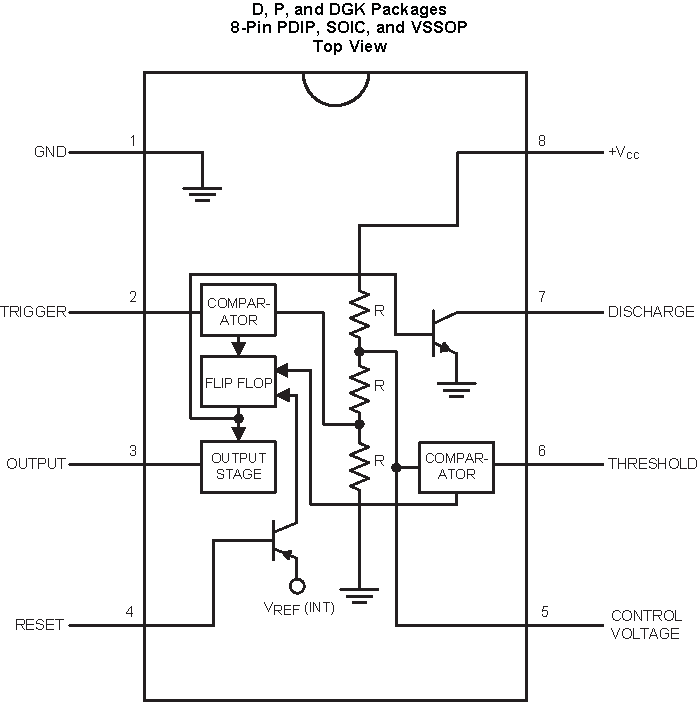
\includegraphics[width=0.8\linewidth]{img/diagrama_lm555.pdf}
  \caption{Diagrama de pinagem do circuito integrado LM555.}
  \label{fig:0}
\end{figure}
\begin{figure}[htpb]
  \centering
  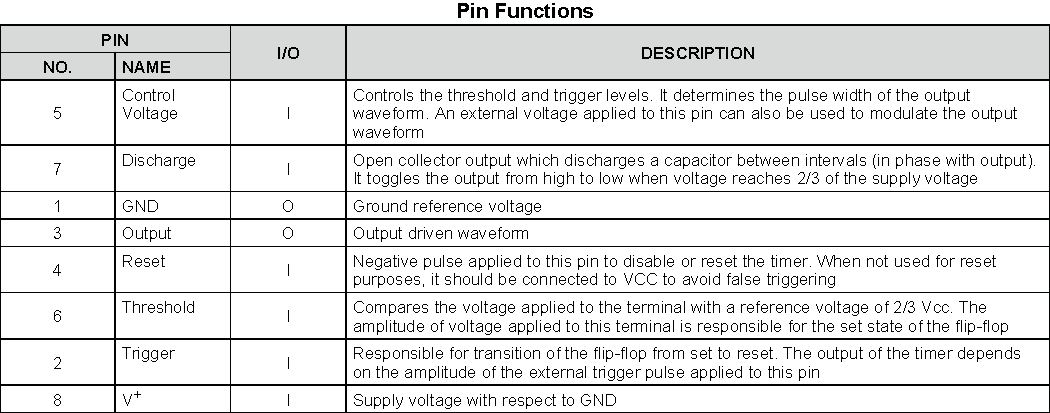
\includegraphics[width=\linewidth]{img/funcoes.pdf}
  \caption{Tabela retirada do datasheet do LM555 (Texas Instrument) com as funções de cada pino.}
  \label{tab:1}
\end{figure}
\subsection{Análises}
No experimento 1, escolhemos os valores de resistência  e capacitância adequado a fim de obter um pulso de duração previamente escolhida, no caso $1s$. Os valores foram de $R=10k \Omega$ e $100\mu F$. Estes valores foram escolhidos através do datasheet que determinava que a duração do pulso é dado por:
\begin{align*}
  t= 1.1 R C = 1.1 \times 10^{4} \times 100\times10^{-6}= 1.1 s
\end{align*}
E foram validados através da montagem do circuito.   O resultado se encontra na Figura~\ref{fig:1}
\begin{figure}[htpb]
  \centering
  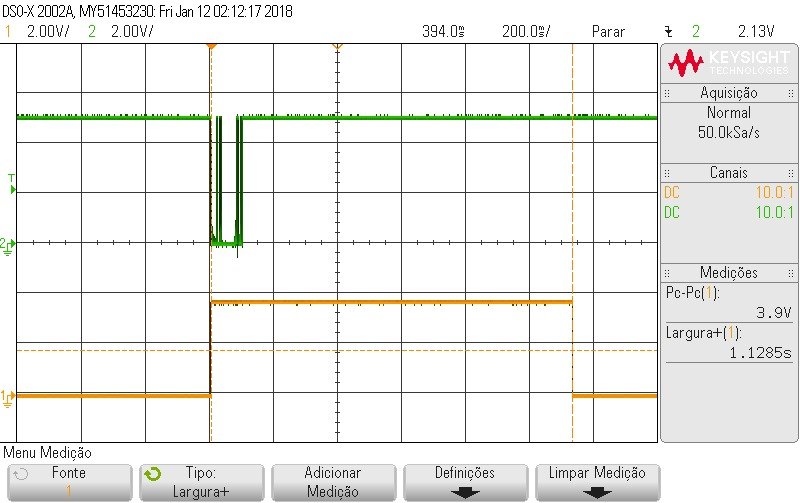
\includegraphics[width=0.8\linewidth]{img/exp1.jpg}
  \caption{Saída do circuito multivibrador monoestável descrito pela Figura~1.}
  \label{fig:1}
\end{figure}

No experimento 2, montou-se o circuito descrito na Figura~2 e com o potenciômetro configurado com seu valor mínimo e seu valo máximo foram obtidos os gráficos das Figuras~\ref{fig:2}-\ref{fig:3}.
\begin{figure}[htpb]
  \centering
  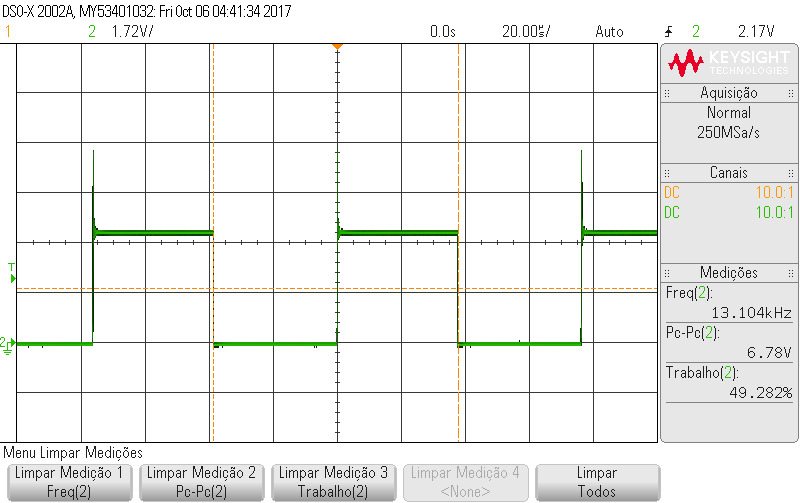
\includegraphics[width=0.8\linewidth]{img/max.jpg}
  \caption{Saída do circuito oscilador descrito na Figura~2, com o potenciômetro em seu valor mínimo. }
  \label{fig:2}
\end{figure}
Observamos que na prática as frequência variaram de $1.82 kHz$ até $13.1khz$. O valor teórico da frequência segundo o datasheet da fabricante texas instrument é dado por:
\begin{align}
  \label{eq:0}
  f= \frac{1.44 }{ \left( R_a + 2 R_B  \right) C } 
\end{align}

O valor minímo de resistência do potenciômetro é em torno de $170 k\Omega$ e o valor máximo é de $1 m\Omega$ ambos somados ao valor fixo de  $ 1.5k\Omega$. A capacitância no circuito vale $390pF$.
\begin{align*}
  F_{min} = \frac{1.44}{10^3 \left(1+ 2 \left(   10^3 +1.5 \right)\right)390\times 10^{-12}}=1.842 \text{kHz}  \\ 
  F_{max} = \frac{1.44}{10^3 \left(1+ 2 \left(   170 +1.5  \right)\right)390\times 10^{-12}}=10.733 \text{kHz}
\end{align*}

Percebe-se assim, que a faixa de frequência possível teórica(1.8 kHz até 10.7 kHz) é menor que a observada na prática (1.8 kHz até 13.1kHz), e provavelmente advém de uma  abordagem mais conservadora do limites de funcionamento do circuito.

Podemos também estimar o ciclo de trabalho com a seguinte equação apresentada no datasheet:

\begin{align}
  D= \frac{R_B}{R_A + 2R_B} 
\end{align}
\begin{align*}
  D_{1}= \frac{1.5 + 10^3}{1+2\times(1.5+10^3)}= 49.975\% \\
  D_{2}= \frac{1.5 + 170}{1+2\times(1.5+170)}= 49.854\% \\
\end{align*}

Percebemos aqui, que tanto na nossa estimativa teórica e experimento prático, maiores valores de 
resistência $R_B$ implicaram em um duty cycle mais próximo de 50\%.
\begin{figure}[htpb]
  \centering
  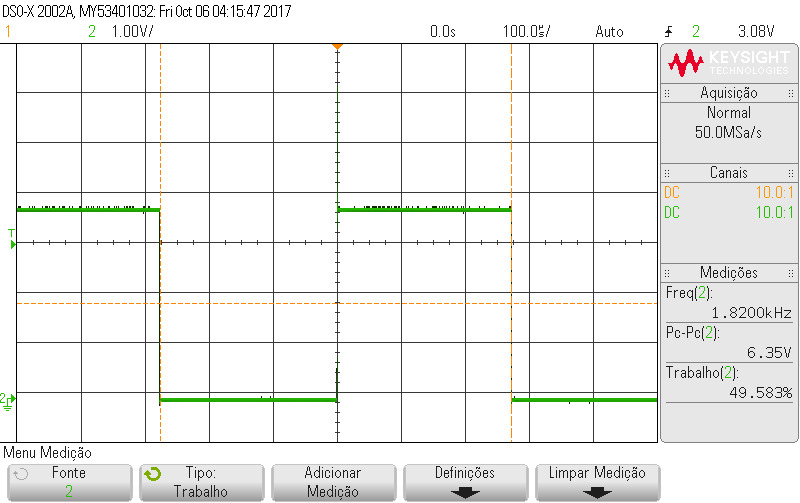
\includegraphics[width=0.8\linewidth]{img/min.jpg}
  \caption{Saída do circuito oscilador descrito na Figura~2, com o potenciômetro em seu valor máximo. }
  \label{fig:3}
\end{figure}
\subsection{Discussões}
No circuito da Figura~1 o circuito integrado LM555 age como um timer que gera um único pulso a cada \emph{trigger}. O capacitor externo é inicialmente tido 
como descarregado pelo transistor dentro do timer.
O pulso de saída começa quando o LM555 recebe um sinal, na pinagem do trigger (pino 2), 
de tensão menor que $1/3$ da tensão da fonte de alimentação. Isto faz com quem o flip-flop mude para o estado de \emph{set} o que descarrega o curto circuito através do capacitor 
e coloca a saída em estado alto.
A tensão sobre o capacitor então cresce exponencialmente pelo período de $t= 1.1 RC$ até que se iguala a $2/3$ do valor da fonte de alimentação. 
Assim, a largura do pulso de saída é determinado pela constante de tempo da rede $RC$, podendo ser extendido ou diminuído para cada aplicação apenas ajustando os valores de $R$ e $C$. 

No experimento da Figura~2, o circuito se comporta como um oscilador, gerando uma onda quadrada de frequência definida pela Equação~\ref{eq:0}. O capacitor externo ao circuito($390pF$) carregará através de $R_A$ e $R_B$, e descarregará por $R_B$. 
A frequência pode ser ajustada de forma precisa pela razão dos dois resistores. Observamos na Figura~\ref{fig:2} e Figura~\ref{fig:3} que a frequência aumentou por um fator
de aproxidamente 7 vezes, o que é coerente com nossas expectativas, já que o valor mínimo do potenciômetro é perto de $170 k\Omega$.
\newpage
\subsection{Conclusão}
Desta prática pôde-se aprender a cerca da utilidade e funcionamento de circuitos multivibradores astáveis e monoestáveis, e como implementá-los com um circuito integrado LM555.  Se tratando do circuitos multivibradores monoestáveis, aprendeu-se como ajustar a largura do pulso
para um valor desejado através da constante de tempo $RC$ e o porquê desta configuração funcionar. Em relação aos circuitos multivibradores astáveis, aprendeu-se como configurar uma frequência desejada através dos resistores ($R_A, R_B$) do circuito e que valores maiores de $R_B$ implicam em duty cycles mais próximos de 50\%, além do porquê desta configuração funcionar.

\end{document}
